\documentclass[10pt,a4paper]{article}
\usepackage[utf8]{inputenc}
\usepackage{amsmath}
\usepackage{amsfonts}
\usepackage{amssymb}
\usepackage{graphicx}
\author{Pranav}
\title{Orbits of Comets}
\begin{document}
\maketitle

You have to make use of the various ODE algorithm on the two-body problem of comet and sun.Investigate the effect of using various algorithms for the problem. Your final output should be plots of the comet's trajectory and the plot of the energy of he comet(Plot Potential Energy,Kinetic Energy and Total Energy in one plot) for each algorithms. Play around with the time step as well.

\subsection*{The Steps}
\begin{enumerate}
\item Set initial position and velociy of the comet
\item Set physical parameters(M,G,C,etc..)
\item Loop over desired number of steps and use the choice of algorithm.Also record the position and energy for ploting
\item Graph the trajectory of the comet
\item Graph the energy of the comet versus time.
\end{enumerate}


\begin{figure}
\centering
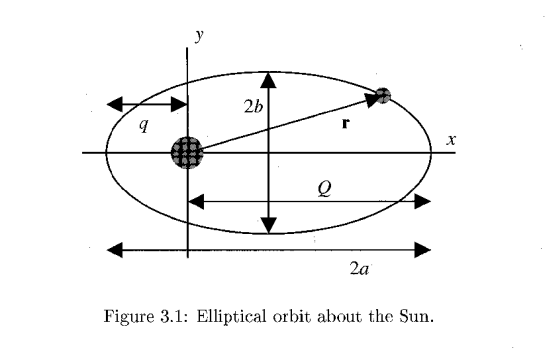
\includegraphics[scale=0.5]{cometorbit.png}
\end{figure}


\begin{figure}
\centering
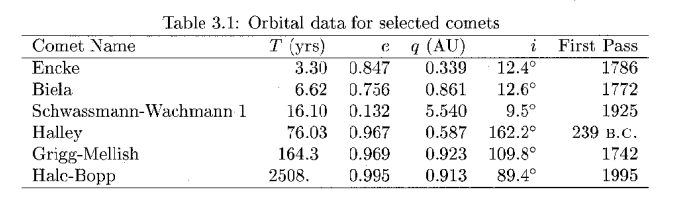
\includegraphics[scale=0.5]{orbitdata.png}
\end{figure}
\end{document}
